\section{Lines \& Planes as VVFs}
\noindent
VVFs are parametric equations that take one input value and return one or more output values as a vector. We can draw curves in space by defining the tail of the output of the VVF be at the origin and have the tip trace out the curve. We will look at some simple VVFs that you need to be able to recognize.\\
\subsection{Lines}
\noindent
A straight line is probably the simplest 3D VVF. We can form any straight line using a point that the line passes through and the direction vector of the line.\\
Letting $P$ be the point and $\vec{v}$ be the direction, a straight line has the form $\vec{r}(t) = \vec{P}+t\vec{v}$, where $\vec{P}$ is the vector with components the same as $P$. The function's output starts at $\vec{P}$ when $t=0$ and moves in the direction of $\vec{v}$ as $t$ increases.

% It'd be nice if we could get this image to fit on the above page
\begin{figure}[h]
	\centering
	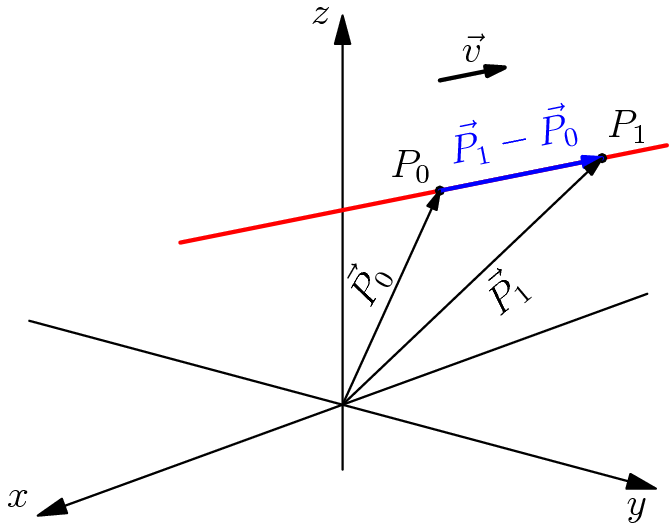
\includegraphics[scale=0.33]{Images/vectorValuedFunctions/VectorLine}
\end{figure}

\noindent
A line can also be formed using two points. To find the equation of the line in this case, let $\vec{v}$ be the vector connecting the two points, and let $\vec{P}$ be a vector point from the origin to one of the two points. We now have an origin point and direction and can write our function as
\begin{equation*}
	\vec{r}(t) = \vec{P_0} + t\left(\vec{P_1} - \vec{P_0}\right)	
\end{equation*}
 Where $P_0$ and $P_1$ are the two points on the line.
\subsection{Planes}
\noindent
A plane can also be formed using a point in the plane, $P$, and a vector perpendicular to the plane, $\vec{n}$. All vectors $\langle x,y,z \rangle$ that originate from $P$ and remain in the plane must be perpendicular to $\vec{n}$, so their dot product with $\vec{n}$ would be 0. So, the point-normal form of a plane is $\vec{n}\cdot\left(\langle x,y,z \rangle - \vec{P}\right) = 0$.\\
\small{Note: Conventionally, $\vec{n}$ is a unit vector, $\hat{n}$.}

\begin{figure}[h]
	\centering
	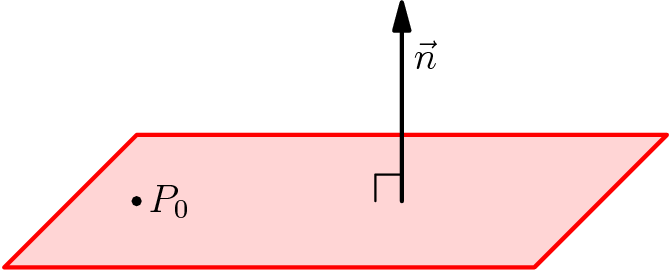
\includegraphics[scale=0.5]{Images/vectorValuedFunctions/PlaneNormalVector}
\end{figure}

\noindent
One can also construct a plane from 3 non-collinear points in the plane. One can still take advantage of point-normal form here by choosing 1 point to be $P_0$ and drawing vectors from this point to the two other points. The cross product of these two vectors is $\vec{n}$. $\left(\left(\vec{P_1} - \vec{P_0}\right) \times \left(\vec{P_2} - \vec{P_0}\right)\right) \cdot \left(\langle x,y,z \rangle - \vec{P_0}\right) = 0$ where $P_0$, $P_1$, and $P_2$ are the three points in the plane.\\

\noindent
One can also construct a plane from a point in the plane, $P_0$, and a line in the plane, $\vec{r}(t) = \vec{P_1} + t\vec{v}$, that doesn't pass through $P_0$. One can get this setup into point-normal form by choosing a an output of $\vec{r}(t)$, like $\vec{P_1}$, and constructing a vector that points from $\vec{P_1}$ to $\vec{P_0}$, $\vec{P_1}-\vec{P_0}$, and crossing this with $\vec{v}$ to find $\vec{n}$. $\left(\vec{v} \times \left(\vec{P_1} - \vec{P_0}\right)\right) \cdot \left(\langle x,y,z \rangle - \vec{P_0}\right) = 0$.\\

\noindent
One can also construct a plane from two intersecting lines, $\vec{r_1}(t) = \vec{P_0} + t\vec{v_1}$ and $\vec{r_2}(t) = \vec{P_0} + t\vec{v_2}$, where $P_0$ is where the two lines intersect. One can cross $\vec{v_1}$ with $\vec{v_2}$ to get the normal vector.
$\left(\vec{v_1} \times \vec{v_2}\right) \cdot \left(\langle x,y,z \rangle - \vec{P-0}\right) = 0$.